 \thispagestyle{gocconone}
\pagestyle{gocco}
\everymath{\color{gocco}}
\graphicspath{{../gocco/pic/}}
\blfootnote{$^1${\color[named]{gocco}Đại kiện tướng quốc tế.}}
\begingroup
\AddToShipoutPicture*{\put(0,616){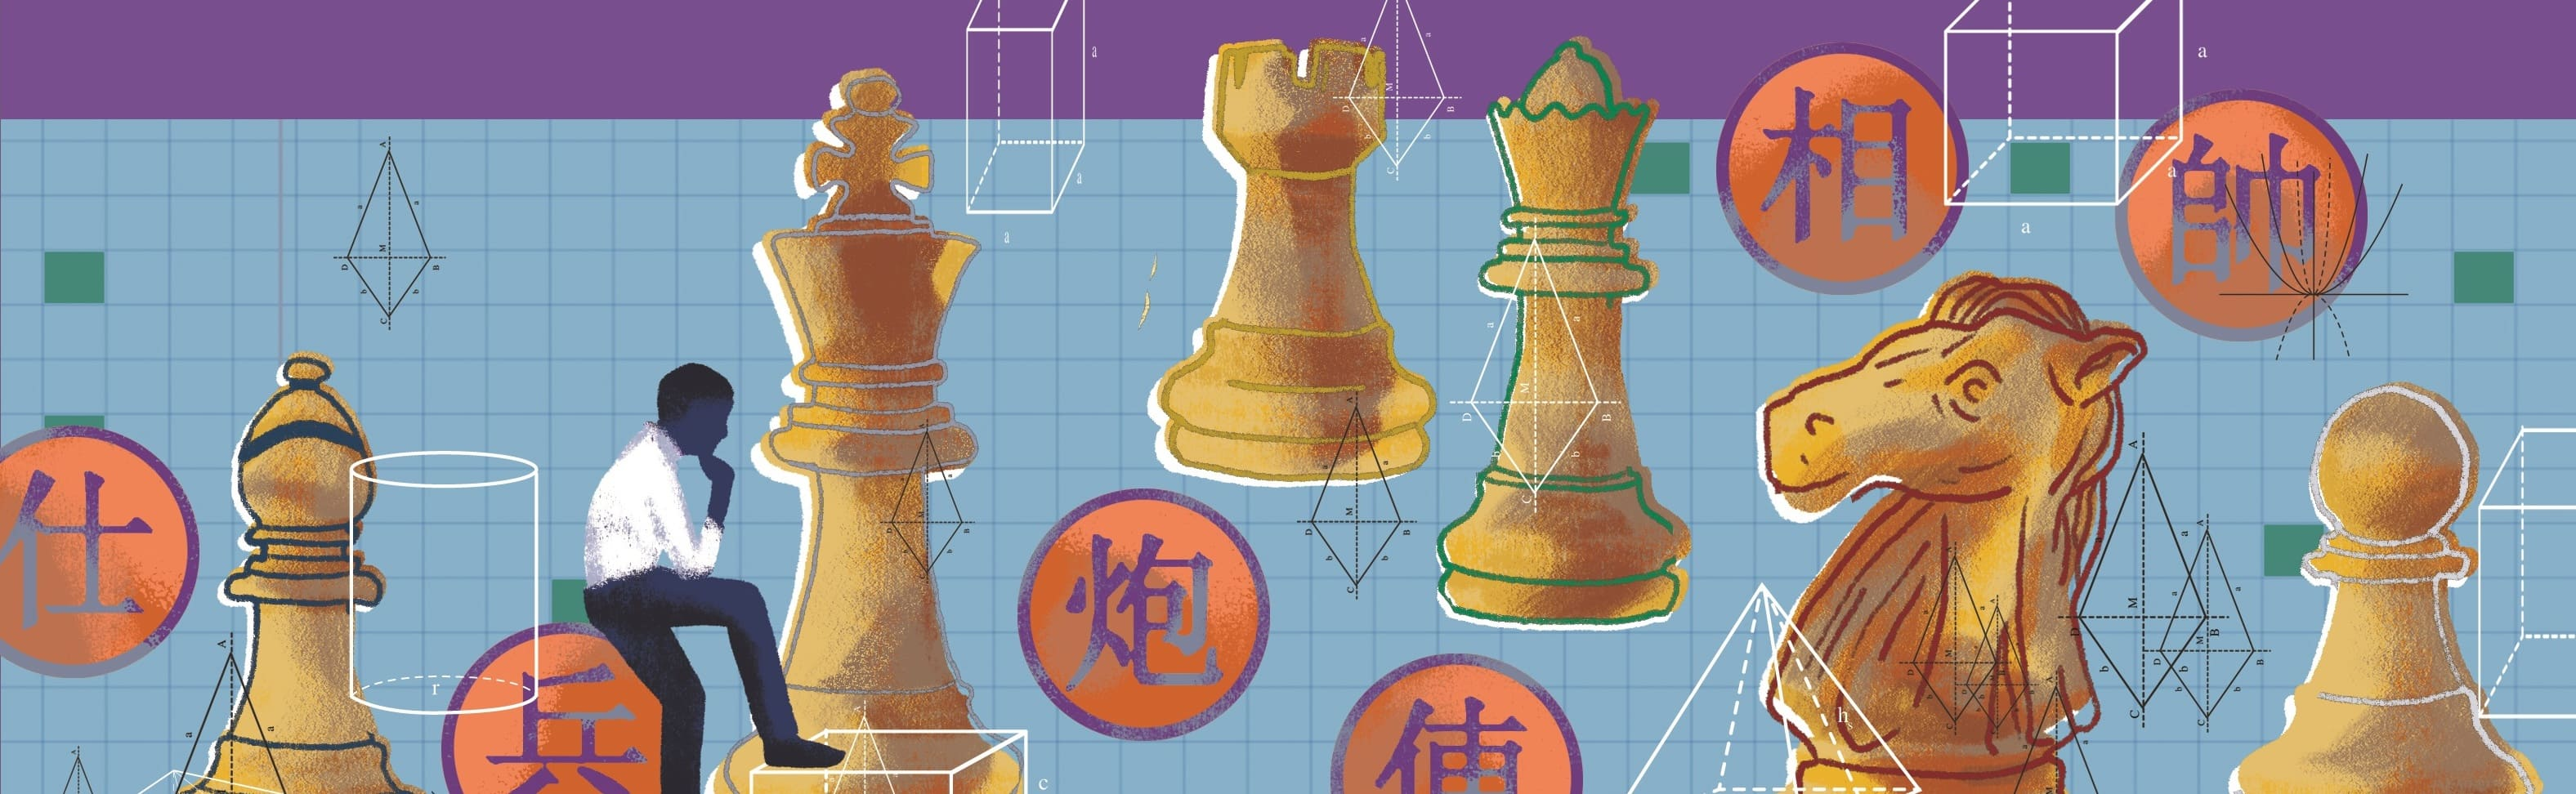
\includegraphics[width=19.3cm]{../bannergocco}}}
\AddToShipoutPicture*{\put(143,558){
\includegraphics[scale=1]{../tieude2.pdf}}} 
\centering
\endgroup

\vspace*{150pt}
\begin{multicols}{2}
	Lý thuyết cơ bản của cờ tàn Xe chống Mã khi hai bên không còn tốt thường được đánh giá là hòa cờ cơ bản. Nếu như Vua và Mã luôn đứng cạnh nhau hoặc ở giữa bàn cờ, bên có Xe không thể giành chiến thắng. Tuy nhiên trên thực tế rất nhiều các kỳ thủ rất mạnh cũng đôi khi mắc phải những sai lầm nghiêm trọng trong thi đấu dẫn đến thua cờ.
	\vskip 0.05cm
	Trong bài viết này, chúng tôi sẽ trình bày hai tình huống cơ bản trong cuộc chiến giữa Xe và Mã.
	\vskip 0.05cm
	-- Trường hợp Vua và Mã đối phương nằm ở hàng ngang cuối $1$ và $8$ hoặc ở cột $a$ và $h$.
	\vskip 0.05cm
	-- Mã bị tách rời khỏi Vua.
	\vskip 0.05cm
	Trong phần I bài viết này, chúng ta sẽ xem xét một số trường hợp khi Vua và Mã đối phương nằm ở hàng ngang cuối $1$ và $8$ hoặc ở cột $a$ và $h$.
	\vskip 0.05cm
	\textbf{\color{gocco}Kling -- Horwitz} $\pmb{(1851)}$
	\begin{center}
		\newgame
		\fenboard{5nk1/4R3/8/6K1/8/8/8/8 b Q - 0 1}
		\scalebox{0.85}\showboard
		\vskip 0.1cm
		\textit{\small\color{gocco}Hình $1$. Trắng đi trước.}
	\end{center}
	\textbf{\color{gocco}$\pmb{1.}$Vf$\pmb{6}$ Mh$\pmb{7+}$ $\pmb{2}$.Vg$\pmb{6}$ Mf$\pmb{8+}$ $\pmb{3}$.Vh$\pmb{6}$ Vh$\pmb{8}$ $\pmb{4}$.Xf$\pmb{7}$ Vg$\pmb{8}$ $\pmb{5}$.Xg$\pmb{7+}$ Vh$\pmb{8}$ $\pmb{6}$.Xg$\pmb{1}$ Md$\pmb{7}$!} [Phương án khác $6$...Me$6$? $7$.Vg$6$ Vg$8$ (\textit{$7$...Mf$4+$ $8$.Vf$7$}) $8$.Vf$6+$; $6$...Mh$7$ $7$.Vg$6$ Vg$8$ (\textit{$7$...Mf$8+$ $8$.Vf$7$ Mh$7$ $9$.Xg$8\#$}) $8$.Xg$2$ Mf$8+$ $9$.Vf$6+$ Vh$8$ $10$.Vf$7$ Mh$7$ $11$.Xg$8\#$]
	\vskip 0.1cm
	\textbf{\color{gocco}$\pmb{7}$.Vg$\pmb{6}$ Vg$\pmb{8}$ $\pmb{8}$.Xf$\pmb{1}$ Mf$\pmb{8+}$ $\pmb{9}$.Vf$\pmb{6}$ Mh$\pmb{7+}$ $\pmb{10}$.Ve$\pmb{7}$ Vg$\pmb{7}$ $\pmb{11}$.Xg$\pmb{1+}$ Vh$\pmb{6}$ $\pmb{12}$.Vf$\pmb{7}$ Mg$\pmb{5+}$ $\pmb{13}$.Vf$\pmb{6}$ Mh$\pmb{7+}$ $\pmb{14}$.Vf$\pmb{5}$ Mf$\pmb{8}$!} Mã đen đủ không gian để di chuyển. Trắng không thể làm cách nào bắt được Mã đen. 
	\begin{center}
		\newgame
		\fenboard{5n2/8/7k/5K2/8/8/8/6R1 b Q - 0 1}
		\scalebox{0.85}\showboard
		\vskip 0.2cm
		\textit{\small\color{gocco}Hình $2$.}
	\end{center}
	Ví dụ tiếp  theo (Hình $3$) cho thấy, ngay cả khi Trắng đã ép Vua đối phương vào cạnh bàn cờ. Nếu Mã ở bên cạnh Vua, trắng cũng không thể giành chiến thắng.
	\vskip 0.1cm
	\textbf{\color{gocco}$\pmb{1}$...Mc$\pmb{6}$ $\pmb{2}$.Xc$\pmb{7}$ Md$\pmb{8}$ $\pmb{3}$.Xe$\pmb{7+}$ Vf$\pmb{8}$ $\pmb{4}$.Xd$\pmb{7}$} [Phương án khác dẫn đến hòa cờ $4$.Xe$1$ Mf$7$ $5$.Xa$1$ Ve$8$! $6$.Xa$8+$ Md$8$ =]
	\begin{center}
		\newgame
		\fenboard{3nk3/7R/5K2/8/8/8/8/8 b Q - 0 1}
		\scalebox{0.85}\showboard
		\vskip 0.2cm
		\textit{\small\color{gocco}Hình $3$. Đen đi trước.}
	\end{center}
	\textbf{\color{gocco}$\pmb{4}$...Ve$\pmb{8}$ $\pmb{5}$.Xc$\pmb{7}$ Vf$\pmb{8}$ $\pmb{6}$.Xa$\pmb{7}$ Ve$\pmb{8}$} [Vua đen và Mã ngăn cản Vua trắng tiếp cận]
	\vskip 0.1cm
	\textbf{\color{gocco}Bài tập $\pmb{1}$: Topalov. V, BUL $\pmb{(2740)}$ -- Ding Liren, CHN $\pmb{(2812)}$}
	\vskip 0.1cm
	Giải tưởng niệm Đại kiện tướng Vugar Gashimov  năm $2019$
	\begin{center}
		\newgame
		\fenboard{6K1/5N2/5k2/7r/8/8/8/8 b Q - 0 1}
		\scalebox{0.85}\showboard
		\vskip 0.2cm
		\textit{\small\color{gocco}Hình $4$. Đen đi trước thắng.}
	\end{center}
	\textbf{\color{gocco}Bài tập $\pmb{2}$: Pandavos, E -- Delithanasis, GRE--ch Liosia $\pmb{1991}$}
	\begin{center}
		\newgame
		\fenboard{8/8/8/5k2/3R4/5K2/6n1/8 b Q - 0 1}
		\scalebox{0.85}\showboard
		\vskip 0.2cm
		\textit{\small\color{gocco}Hình $5$. Đen đi trước, hòa.}
	\end{center}
	\columnbreak
	\textbf{\color{gocco}Bài tập $\pmb{3}$: Neumann -- Steinitz, Baden--Baden $\pmb{1870}$}
	\begin{center}
		\newgame
		\fenboard{5KN1/1r6/4k3/8/8/8/8/8 b Q - 0 1}
		\scalebox{0.85}\showboard
		\vskip 0.2cm
		\textit{\small\color{gocco}Hình $6$. Trắng đi trước, hòa.}
	\end{center}
	\textbf{\color{gocco}Bài tập $\pmb{4}$: Geller -- A.Rodriguez, Amsterdam II $\pmb{1987}$.}
	\begin{center}
		\newgame
		\fenboard{6k1/4R3/8/6Kn/8/8/8/8 b Q - 0 1}
		\scalebox{0.85}\showboard
		\vskip 0.2cm
		\textit{\small\color{gocco}Hình $7$. Đen đi trước, hòa.}
	\end{center}
%	\textbf{\color{gocco}Lời giải:} 
%	\vskip 0.1cm
%	\textbf{\color{gocco}Bài $\pmb{1}$: $\pmb{1}$...Xd$\pmb{5}$!! $\pmb{2}$.Mh$\pmb{6}$} [$2$.Vf$8$ Xd$7$]
%	\vskip 0.1cm
%	\textbf{\color{gocco}$\pmb{2}$...Xd$\pmb{8+}$ $\pmb{3}$.Vh$\pmb{7}$ Xd$\pmb{7+}$ $\pmb{4}$.Vg$\pmb{8}$ Vg$\pmb{6}$}
%	\vskip 0.1cm
%	$0-1$
%	\vskip 0.1cm
%	\textbf{\color{gocco}Bài $\pmb{2}$: $\pmb{1}$...Ve$\pmb{5}$!!} [Nước đi duy nhất. Phương án khác dẫn đến thua cờ.]
%	\vskip 0.1cm
%	[$1$...Me$1+$ $2$.Vf$2$ Mc$2$ $3$.Xc$4$ Ma$3$ $4$.Xc$3$! Mb$1$ $5$.Xd$3$ Mã đen hết đường di chuyển.]
%	\vskip 0.1cm
%	\textbf{\color{gocco}$\pmb{2}$.Xc$\pmb{4}$} [$2$.Xe$4+$ Cả hai phương án đều dẫn đến hòa cờ vì bên trắng không thể bắt được mã đen. $2$...Vf$5$ (\textit{$2$...Vd$5$})]
%	\vskip 0.1cm
%	\textbf{\color{gocco}$\pmb{2}$...Me$\pmb{1+}$ $\pmb{3}$.Vf$\pmb{2}$ Vd$\pmb{5!}$ $\pmb{4}$.Xc$\pmb{3}$ Vd$\pmb{4}$!} [Mã đen trốn thoát.]
%	\vskip 0.1cm
%	$1/2 -1/2$
%	\vskip 0.1cm	
%	\textbf{\color{gocco}Bài $\pmb{3}$: $\pmb{1}$.Mh$\pmb{6}$ Xh$\pmb{7}$ $\pmb{2}$.Mg$\pmb{8}$! Rb$\pmb{7}$ $\pmb{3}$.Mh$\pmb{6}$ Vf$\pmb{6}$ $\pmb{4}$.Mg$\pmb{8}$ Ve$\pmb{6}$ $\pmb{5}$.Mh$\pmb{6=}$}
%	\vskip 0.1cm
%	$1/2 -1/2$
%	\vskip 0.1cm
%	\textbf{\color{gocco}Bài $\pmb{4}$: $\pmb{1}$...Vf$\pmb{8}$! $\pmb{2}$.Xd$\pmb{7}$ Mg$\pmb{7}$ $\pmb{3}$.Vg$\pmb{6}$ Me$\pmb{8}$! $\pmb{4}$.Xf$\pmb{7+}$ Vg$\pmb{8}$ $\pmb{5}$.Xe$\pmb{7}$ Kf$\pmb{8}$! $\pmb{6}$.Xd$\pmb{7}$ Vg$\pmb{8}$! $\pmb{7}$.Xf$\pmb{7}$ Md$\pmb{6}$ $\pmb{8}$.Xf$\pmb{6}$ Me$\pmb{8}$! $\pmb{9}$.Xf$\pmb{1}$ Mg$\pmb{7}$ $\pmb{10}$.Vf$\pmb{6}$ Mh$\pmb{5+}$ $\pmb{11}$.Vg$\pmb{5}$ Mg$\pmb{7=}$ $\pmb{12}$.Vg$\pmb{6}$ Me$\pmb{8}$ $\pmb{13}$.Xf$\pmb{3}$ Mc$\pmb{7}$! $\pmb{14}$.Xf$\pmb{2}$} [$14$.Xc$3$ Me$8$ $15$.Xc$8$ Vf$8=$ Trắng không có cách nào bắt được mã đen]
%	\vskip 0.1cm
%	\textbf{\color{gocco}$\pmb{14}$...Ne$\pmb{8=}$} 
%	\vskip 0.1cm
%	$1/2 -1/2$
\end{multicols}




